\documentclass[12pt]{article}

\usepackage{graphicx}% Include figure files
\usepackage{dcolumn}% Align table columns on decimal point

% Use Arial font %
\usepackage{helvet}
\renewcommand{\familydefault}{\sfdefault} 

% Default margins and paper properties %
\usepackage[a4, portrait, margin=0.6in]{geometry}

\begin{document}
	\title{Hypothesis plots summary} % Force line breaks with \\
	\author{1666957, Gustavo Espinal Lugo}
	\date{\today} % It is always \today, today, %  but any date may be explicitly specified

	\maketitle
	%\tableofcontents
	
	\section*{Plots and corresponding metadata}
	mean expected W mass: 80.379 $[GeV/c^{2}]$,\\
mean hypothesis masses: [78.  78.5 79.  79.5 80.  80.5 81.  81.5 82. ] $[GeV/c^{2}]$,\\
mass width: 2.07 $[GeV/c^{2}]$,\\
chi\_square value of hypothesis fit: 12.277004393963184\\
	Absolute path to figure: /home/physics/phuxdp/Desktop/PX402 Physics Project/WBosonProject/T2W5/plots/muPT\_80.379\_2.07\_between\_78\_and\_82\_summary.png\\
	Next lines are the data of the shown histograms (if needed): \\
	All quantities: 	80.379, [78.  78.5 79.  79.5 80.  80.5 81.  81.5 82. ], 2070, 12.277004393963184\\
	X\_energ\_vls = [0.6, 1.7999999999999998, 3.0, 4.199999999999999, 5.4, 6.6, 7.8, 9.0, 10.2, 11.399999999999999, 12.6, 13.799999999999999, 15.0, 16.2, 17.4, 18.6, 19.799999999999997, 21.0, 22.2, 23.4, 24.6, 25.799999999999997, 27.0, 28.199999999999996, 29.4, 30.6, 31.799999999999997, 33.0, 34.2, 35.4, 36.599999999999994, 37.8, 39.0, 40.2, 41.4, 42.599999999999994, 43.8, 45.0, 46.2, 47.4, 48.599999999999994, 49.8, 51.0, 52.2, 53.4, 54.599999999999994, 55.8, 57.0, 58.199999999999996, 59.4, 60.599999999999994, 61.8, 63.0, 64.19999999999999, 65.4, 66.6, 67.8, 69.0, 70.19999999999999, 71.4, 72.6, 73.8, 75.0, 76.19999999999999, 77.4, 78.6, 79.8, 81.0, 82.19999999999999, 83.4, 84.6, 85.8, 87.0, 88.19999999999999, 89.4, 90.6, 91.8, 93.0, 94.19999999999999, 95.4, 96.6, 97.8, 99.0, 100.19999999999999, 101.4, 102.6, 103.8, 105.0, 106.19999999999999, 107.4, 108.6, 109.8, 111.0, 112.19999999999999, 113.4, 114.6, 115.79999999999998, 117.0, 118.19999999999999, 119.4]\\
	Y\_data\_bin\_cnts = [0.0, 0.0, 0.0, 0.0, 0.0, 0.0, 0.0, 0.0, 0.0, 0.0, 0.0, 0.0, 0.0, 0.0, 0.0, 0.0, 2.6272265911102295, 4.258678436279297, 411.0599060058594, 19834.36328125, 25654.76953125, 27492.1484375, 29399.1171875, 31445.021484375, 33674.59375, 35479.23046875, 37453.0390625, 38995.7890625, 41129.69140625, 41910.35546875, 43507.53125, 43788.16015625, 40698.3125, 34981.6171875, 27335.462890625, 20507.5390625, 15436.955078125, 12118.1220703125, 9656.71875, 7876.9765625, 6411.98046875, 5231.4833984375, 4520.0859375, 3801.73583984375, 3213.220458984375, 2732.826416015625, 2341.7314453125, 2076.64306640625, 1818.6474609375, 1628.831787109375, 1405.4285888671875, 1271.6634521484375, 1088.3131103515625, 942.9937744140625, 903.0429077148438, 757.8724365234375, 706.1197509765625, 623.2659301757812, 536.2207641601562, 473.77142333984375, 468.772705078125, 429.5991516113281, 385.8650207519531, 332.1512756347656, 317.75103759765625, 287.9624328613281, 266.9156494140625, 239.6173858642578, 207.060302734375, 182.9595184326172, 215.72808837890625, 158.14715576171875, 150.80113220214844, 160.19888305664062, 133.1354522705078, 118.35227966308594, 123.95072174072266, 109.80606842041016, 94.69293212890625, 76.50025177001953, 92.15445709228516, 91.18305206298828, 86.8621597290039, 58.849674224853516, 62.39198684692383, 66.516845703125, 51.518882751464844, 46.24637222290039, 49.22967529296875, 47.363338470458984, 35.41771697998047, 42.362308502197266, 34.773494720458984, 35.56611251831055, 28.009634017944336, 32.365970611572266, 31.151290893554688, 30.208356857299805, 33.36943817138672, 16.019208908081055]\\
	Y\_model\_bin\_cnts = [0.0, 0.0, 0.0, 0.0, 0.0, 0.0, 0.0, 0.0, 4.101123332977295, 7.663997173309326, 0.0, 0.0, 0.0, 0.0, 0.0, 1.9238522052764893, 0.0, 8.782835960388184, 374.4552307128906, 19139.666015625, 24711.69921875, 26640.58203125, 28266.40234375, 30119.58203125, 32216.7265625, 34020.58984375, 35966.08203125, 37468.67578125, 39297.79296875, 40811.6484375, 41788.1484375, 41685.3125, 39148.96875, 33170.08984375, 26115.07421875, 19678.041015625, 15072.0615234375, 11797.7021484375, 9252.412109375, 7498.21240234375, 6328.04931640625, 5189.8125, 4367.48388671875, 3598.0341796875, 2962.368408203125, 2669.89111328125, 2334.505615234375, 1975.554443359375, 1694.23193359375, 1519.984619140625, 1283.98291015625, 1220.0179443359375, 1047.61669921875, 962.0630493164062, 797.534423828125, 710.9413452148438, 656.0203247070312, 642.6231079101562, 584.046875, 481.2906494140625, 425.02020263671875, 383.2881774902344, 341.0120544433594, 307.25689697265625, 310.9994812011719, 243.84129333496094, 232.2761688232422, 242.4253692626953, 224.12124633789062, 220.83544921875, 178.28875732421875, 161.1588134765625, 136.97256469726562, 119.9537124633789, 129.80130004882812, 126.69454956054688, 105.55067443847656, 103.23039245605469, 99.6817398071289, 95.34903717041016, 76.10367584228516, 85.2097396850586, 68.81581115722656, 84.99134063720703, 61.82329559326172, 56.138118743896484, 56.03828048706055, 43.4036979675293, 54.45879364013672, 41.66075897216797, 44.19742202758789, 30.37186622619629, 37.68223190307617, 33.90385818481445, 24.18895149230957, 30.970230102539062, 30.146305084228516, 31.00786781311035, 24.082813262939453, 23.796789169311523]\\

    Found optimal massses ($\chi^2$ roots): [80.42277708] $[GeV/c^{2}]$
    Uncertainty [GeV/c^2]: 4.263256414560601e-14

	\begin{figure}[tb]
		\centering
		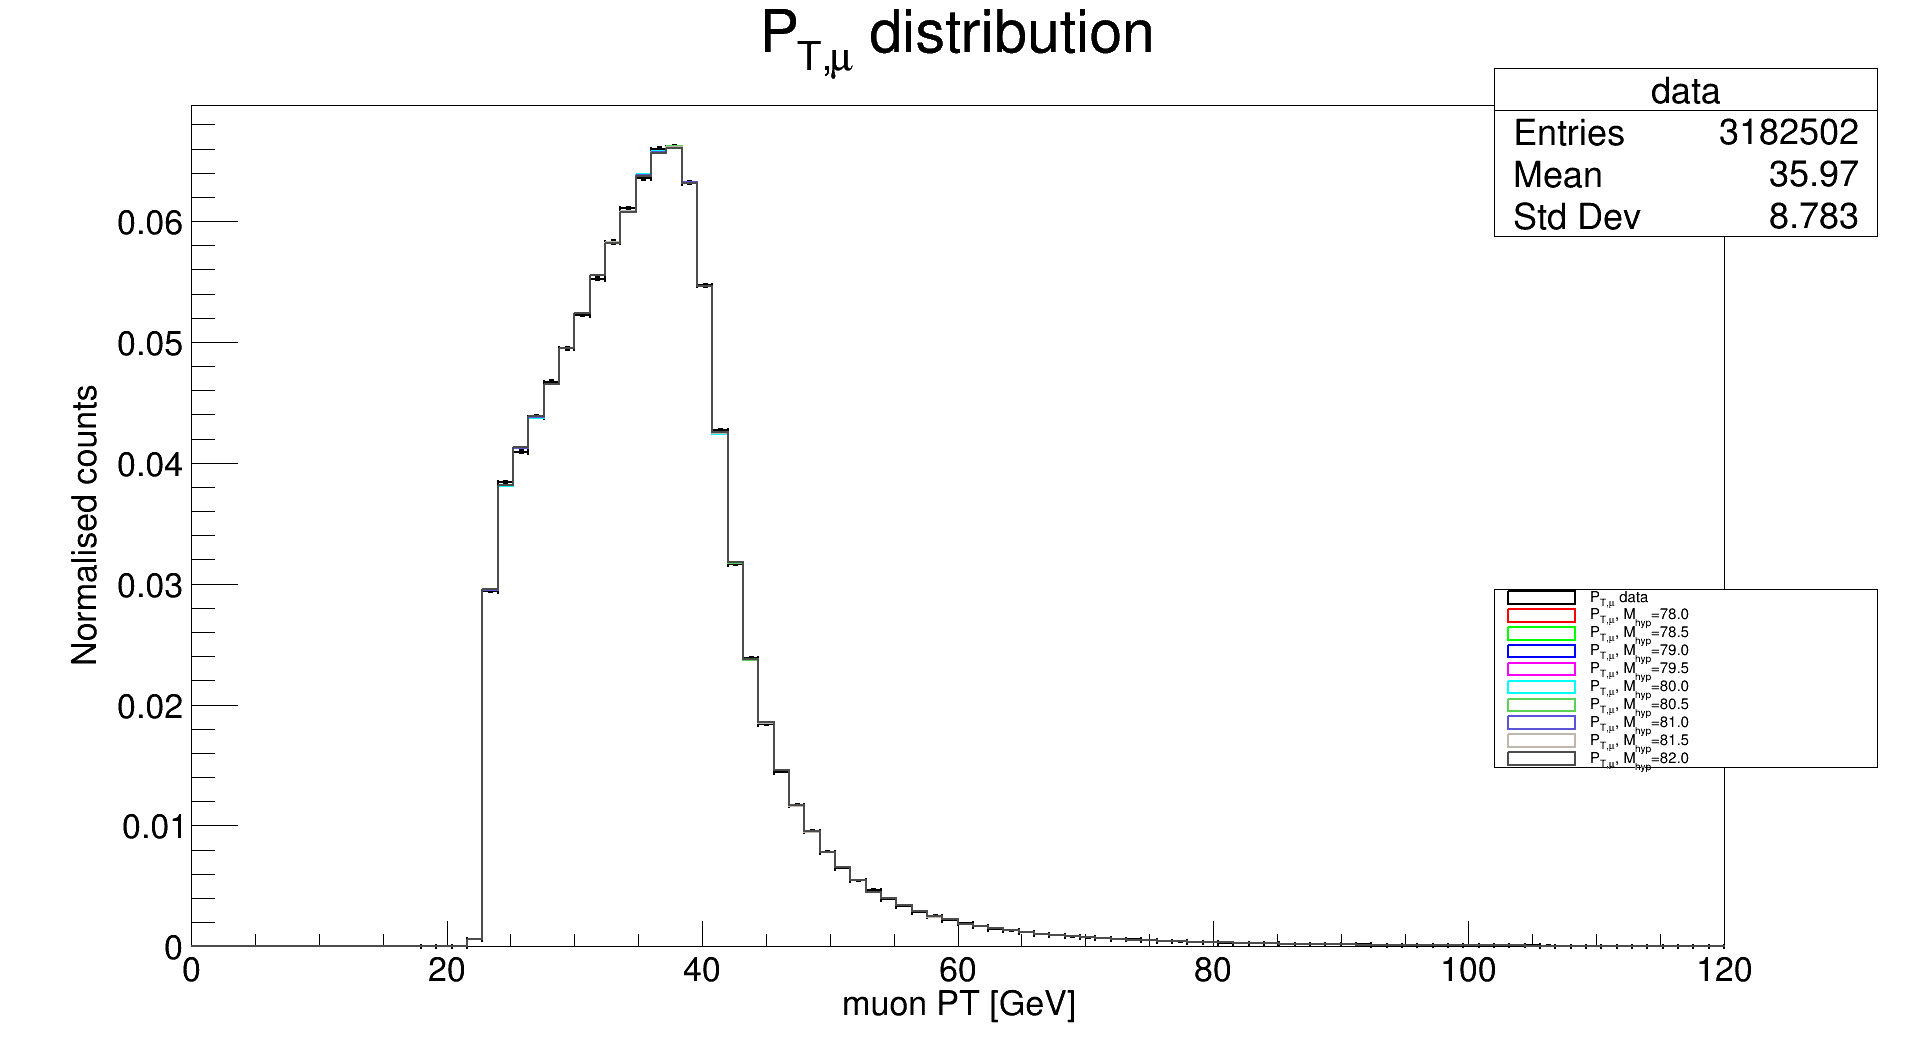
\includegraphics[width=\columnwidth]{/home/physics/phuxdp/Desktop/PX402 Physics Project/WBosonProject/T2W5/plots/muPT_80.379_2.07_between_78_and_82_summary.png}
		\caption{\small Hypothesis masses mean expected W mass: 80.379 $[GeV/c^{2}]$,\\
mean hypothesis masses: [78.  78.5 79.  79.5 80.  80.5 81.  81.5 82. ] $[GeV/c^{2}]$,\\
mass width: 2.07 $[GeV/c^{2}]$,\\
chi_square value of hypothesis fit: 12.277004393963184. }
		\label{fig: fig_0}
	\end{figure}

       \begin{figure}[tb]
		\centering
		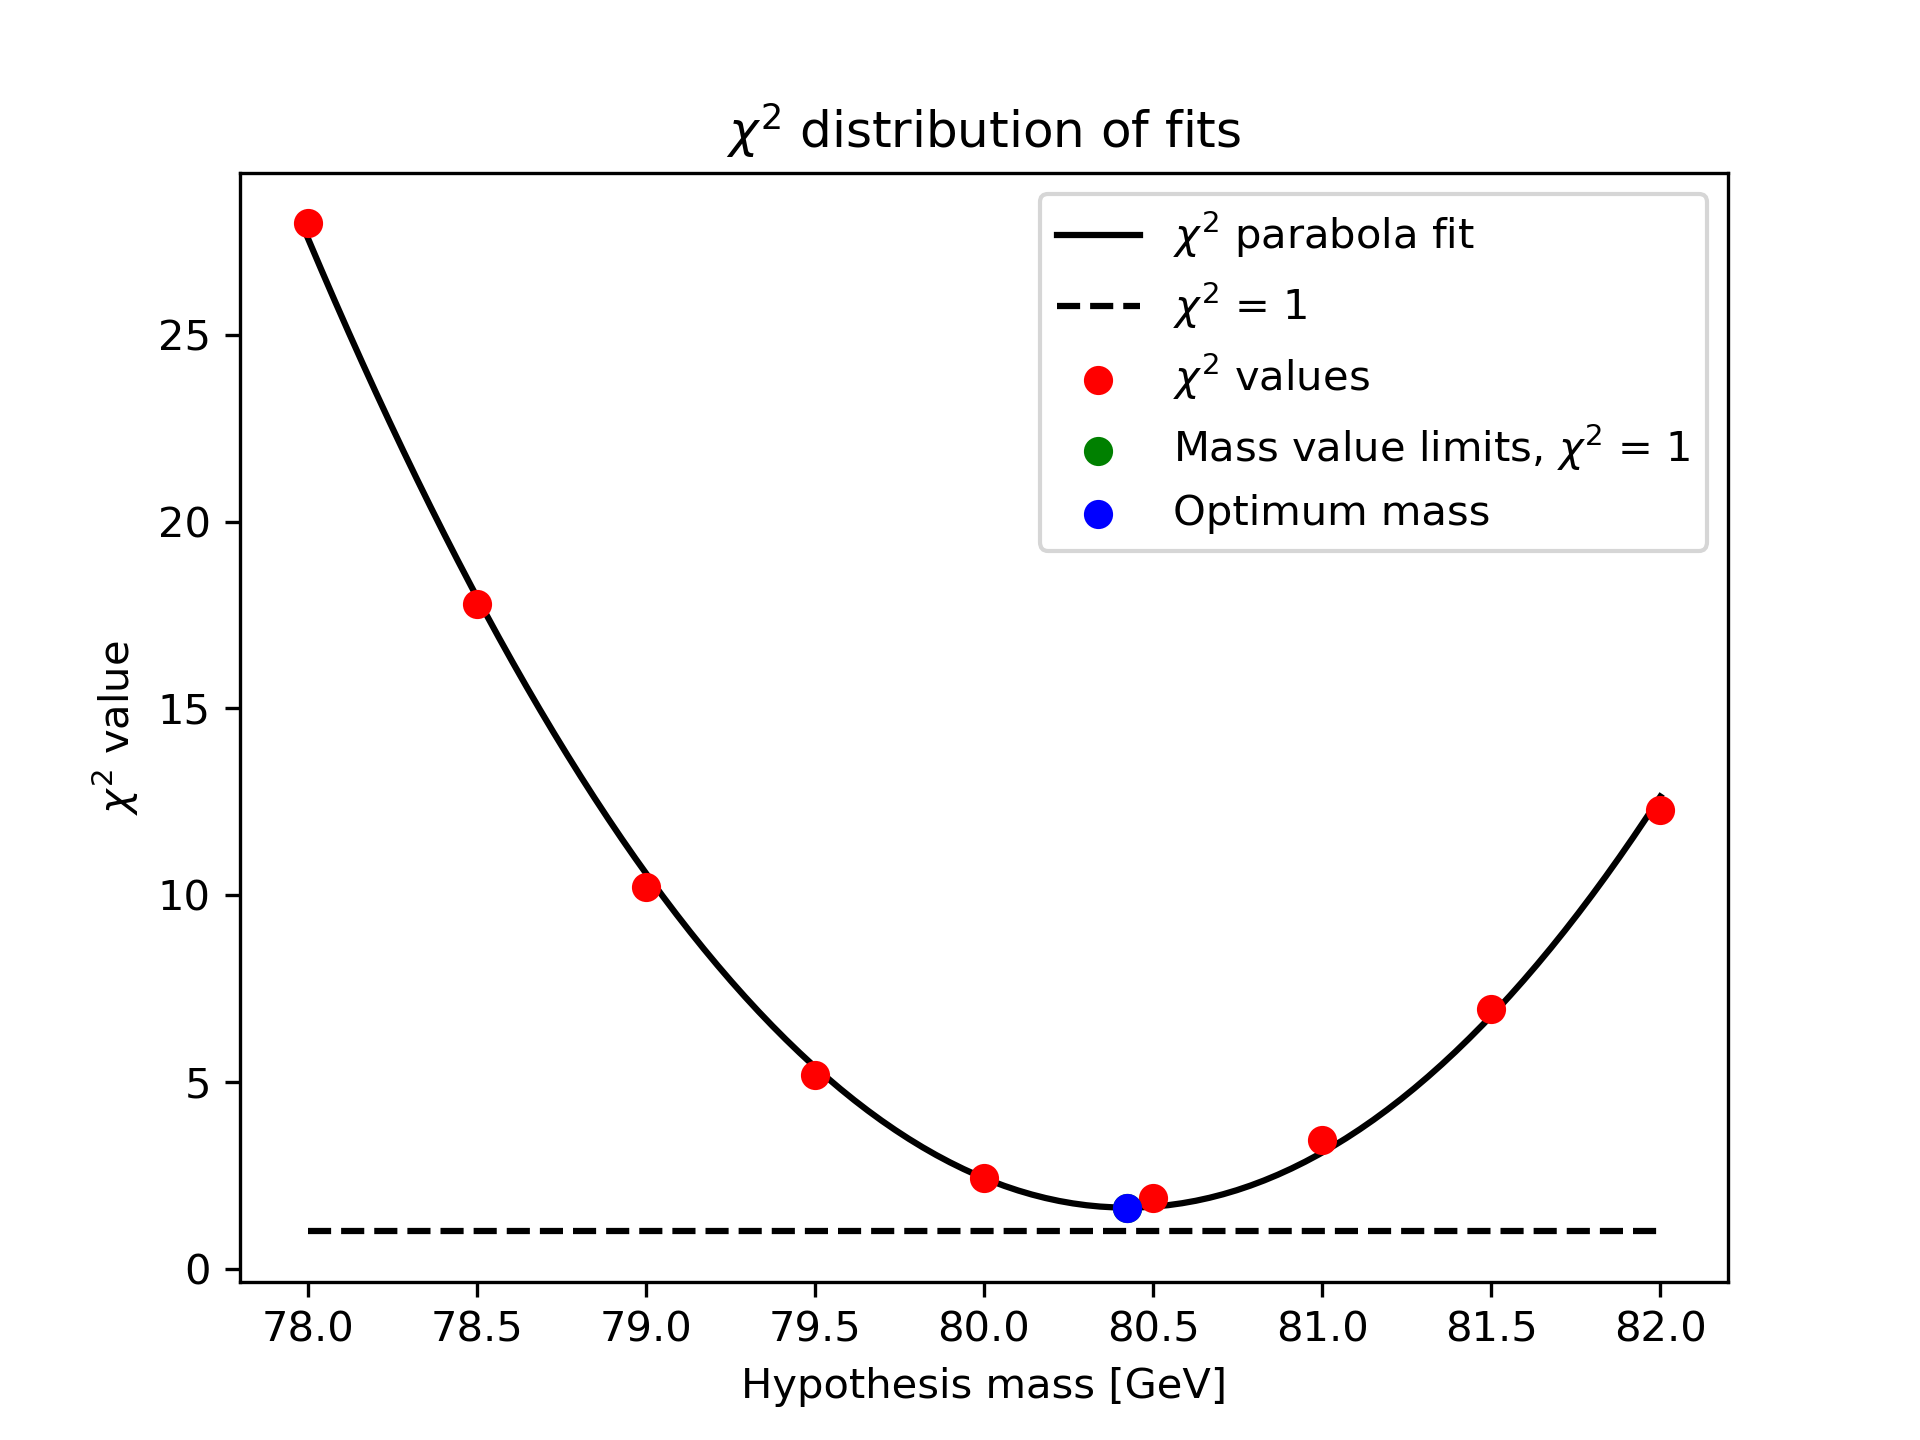
\includegraphics[width=\columnwidth]{/home/physics/phuxdp/Desktop/PX402 Physics Project/WBosonProject/T2W5/plots/chi_square_fits_muPT_80.379_2.07_between_78_and_82_summary.png}
		\caption{\small $\chi^2$ of hypothesis masses. }
		\label{fig: fig_chi_square}
	\end{figure}

    \begin{figure}[tb]
		\centering
		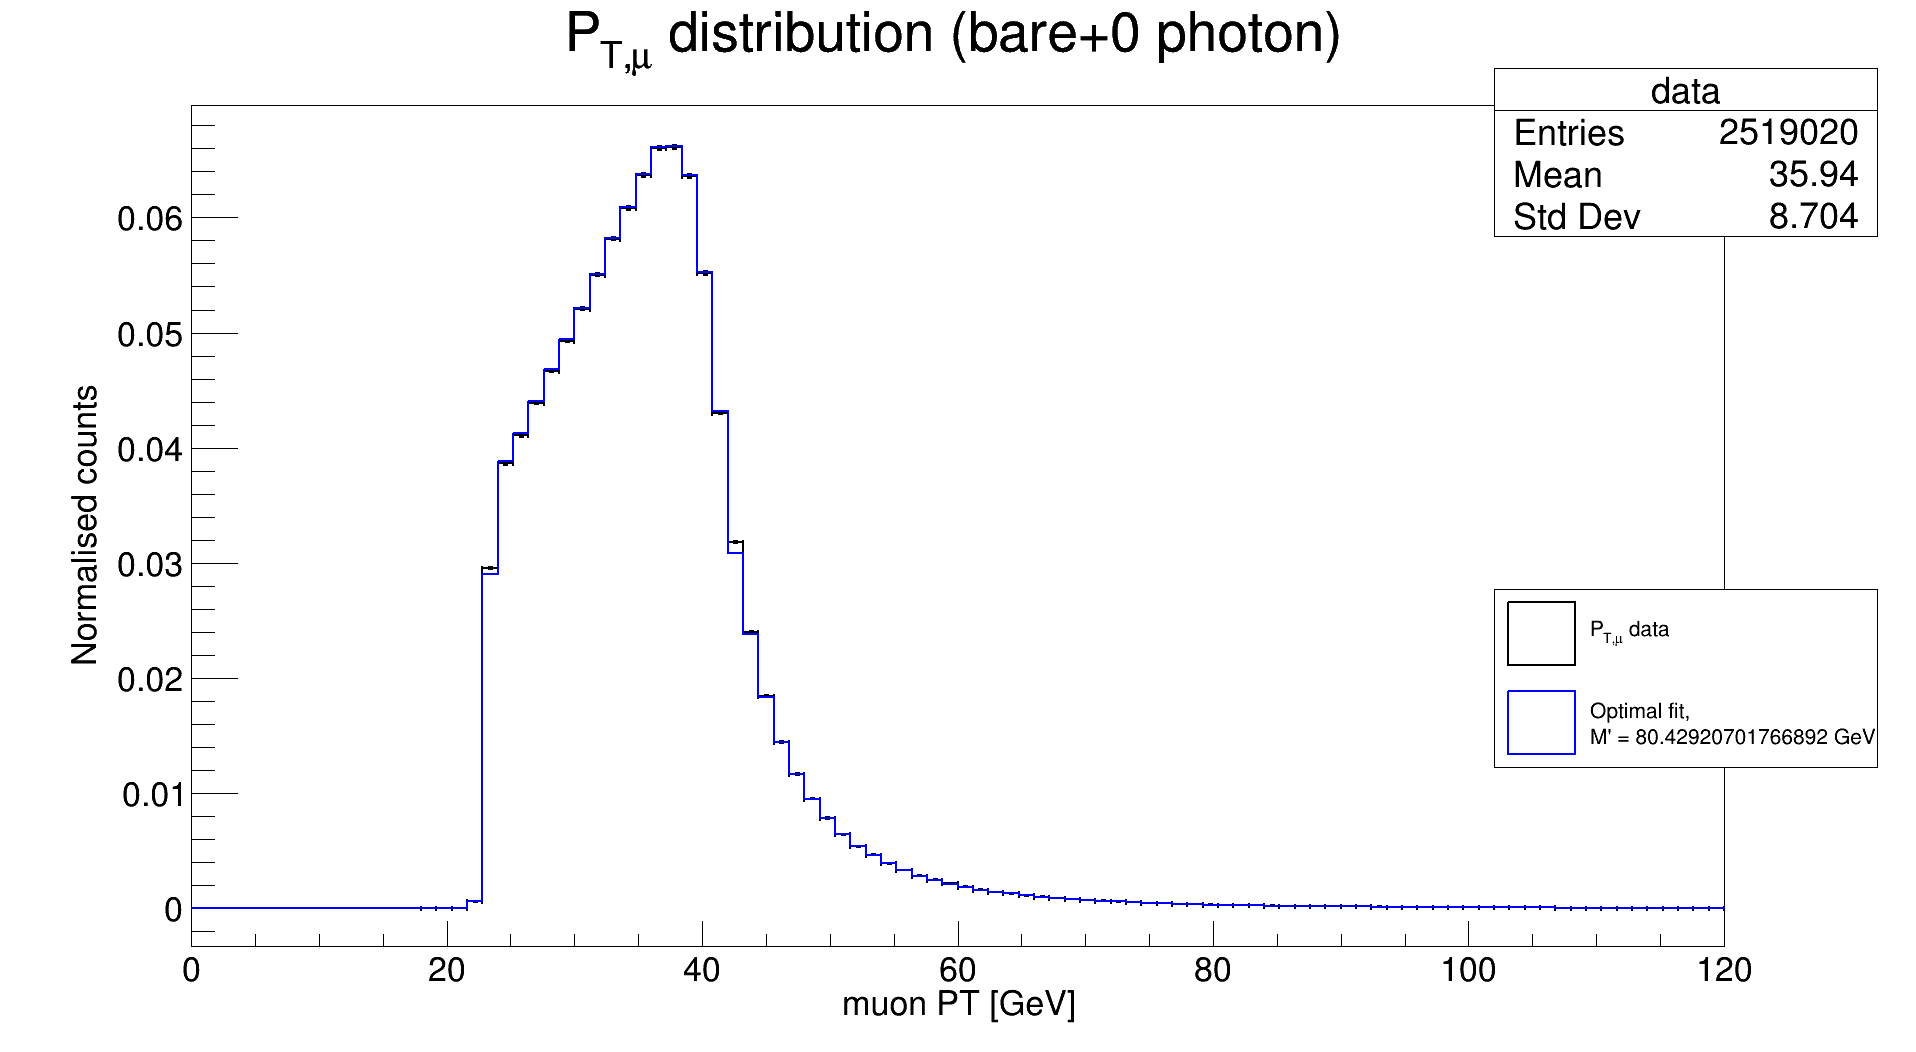
\includegraphics[width=\columnwidth]{/home/physics/phuxdp/Desktop/PX402 Physics Project/WBosonProject/T2W5/plots/optimum_muPT_80.379_2.07_between_78_and_82_summary.png}
		\caption{\small Data and optimum fit with $\chi^2 = 0.024937773839225155$. Used the hypothesis mass of 80.42277708237805$\pm$4.263256414560601e-14 $[GeV/c^{2}]$. }
		\label{fig: fig_optim_parms}
	\end{figure}
    
\end{document}